\documentclass[12pt,lettersize,oneside]{article}
\usepackage[spanish]{babel}
\usepackage[utf8]{inputenc}
\usepackage{amsmath}
\usepackage{amssymb}
\usepackage{fancyhdr}
\usepackage{longtable}
\usepackage{sudoku}
\usepackage[hyphens]{url}
\usepackage{listings}
\lstset{
  language=C,
  basicstyle=\small
}
\usepackage[pdftex]{graphicx}
\usepackage{color}
\definecolor{gray75}{gray}{.75}
\lstdefinestyle{consola}
{basicstyle=\small\bf\ttfamily,
backgroundcolor=\color{gray75},
}
\lstdefinestyle{consola2}
{basicstyle=\footnotesize\bf\ttfamily,
backgroundcolor=\color{gray75},
}
\pagestyle{fancy}


\title{Grupo 3 \\Segunda versión de KECOSATS}
\author{Carlos Colmenares \and Kelwin Fernández \and Eleazar Leal}
\begin{document}
%\maketitle
\setlength{\parskip}{2.5mm}
\setlength{\itemsep}{0ex }
%\tableofcontents

\appendix
\section{Ejecución de KECOSATS}

Seguidamente daremos algunos detalles adicionales sobre la ejecución de
KECOSATS, para así ampliar la información proporcionada en le sección 5.

En la sección 5 se comentó acerca de cómo ejecutar la aplicación, repetiremos
aquí esa información, pero daremos una descripción más detallada de la entrada.


Con la distribución de KECOSATS se incluye entre otras cosas lo siguiente: \vspace{-2.5mm}
\begin{enumerate}
\item Un programa llamado {\tt sudoku} que
realiza lo siguiente:\vspace{-2.5mm}
\begin{itemize}
  \item Recibe un archivo que en cada línea tiene una instancia de Sudoku.
  \item Llama al programa KECOSATS por cada instancia.
  \item Genera automáticamente un archivo {\tt pdf} con la solución.
\end{itemize}
La idea del programa {\tt sudoku} es automatizar la prueba de los 60 casos de
uso.

\item El programa {\tt kec\_o\_sat\_s}, que en este informe hemos llamado
  simplemente KECOSATS, que resuelve instancias de SAT dadas en el
  formato DIMACS.

\item Un archivo {\tt test/sudoku.in} que tiene la lista de las 60 instancias de
  \emph{Sudoku}. La idea de incluir este archivo es suministrarlo como argumento
  al programa {\tt sudoku} para probar automáticamente los 60 casos de prueba de
  \emph{Sudoku} que contiene.
\end{enumerate}

\rule{4cm}{0.3mm}

\textbf{Paso para ejecutar la aplicación {\tt sudoku}:}
\begin{enumerate}
\item Para emplear la aplicación se debe escribir en la consola y desde el directorio
raíz, el siguiente comando tal cual

\begin{lstlisting}[style=consola]
# ./sudoku -f test/sudoku.in -o sudoku.cnf 
           -e solution.pdf -t 100
\end{lstlisting}
\end{enumerate}
donde:
\begin{itemize}
\item {\tt test/sudoku.in} Es un archivo con una lista de instancias de
  \emph{Sudoku} ---los 60 casos por ejemplo. Este archivo consiste de una serie
  de líneas de texto, cada línea representa una instancia de \emph{Sudoku} y
  tiene el formato: 
  {\tt 3 0,2,7,9,4,0,0,0,3,2,...}
  
  donde el primer número es la dimensión del \emph{Sudoku}, y le sigue una lista
  de números separados por comas, que corresponden a la asignación inicial que
  se da a las casillas de la instancia de \emph{Sudoku} a resolver. El tamaño de
  la lista de números separados por comas es el número de casillas de la
  instancia de \emph{Sudoku} que se quiere resolver.

\item {\tt sudoku.cnf} Es el archivo {\tt .cnf} que contiene la formulación
  \emph{SAT} del último caso de prueba que está contenido en {\tt
    test/sudoku.in}.
\item {\tt solution.pdf} Es el nombre del archivo {\tt .pdf} que contendrá las
  soluciones a todas las instancias codificadas en el archivo {\tt
    test/sudoku.in}.
\item{\tt 100} Es el límite de tiempo asignado a la ejecución de cada instancia
  de \emph{Sudoku}.
\end{itemize}

\rule{4cm}{0.3mm}

\textbf{Paso para ejecutar la aplicación {\tt kec\_o\_sat\_s}:}

Nota: En principio, si la idea es probar los 60 casos de prueba de \emph{Sudoku}
contenidos en {\tt test/sudoku.in}, lo ideal sería ejecutar el programa {\tt
  sudoku} tal como se indicó arriba. La ventaja es que {\tt sudoku} genera de
una vez las soluciones en {\tt pdf}.


Para emplear la aplicación, escribir en la consola el comando
\begin{enumerate}
\item \begin{lstlisting}[style=consola]
# kec_o_sat_s -f inputfilename -o outputfilename 
\end{lstlisting}
\end{enumerate}
\noindent donde:
\vspace{-2.5mm}
\begin{itemize}
\item {\tt inputfilename} es el nombre del archivo que contiene la instancia del
  problema SAT a resolver. Esta instancia debe estar en el formato DIMACS.
(Consultar http://logic.pdmi.ras.ru/~basolver/dimacs.html para información sobre
este formato.)
\item {\tt outputfilename} es el nombre del archivo que contendrá los resultados
  generados tras correr el algoritmo.
\end{itemize}


\section{Comentarios adicionales sobre el desempeño de KECOSATS}

A continuación haremos algunos comentarios complementarios acerca del desempeño
de KECOSATS.
\begin{itemize}
\item En la sección anterior que presentó la comparación de desempeño entre
  KECOSATS ---con y sin aprendizaje de cláusulas--- y \emph{zChaff}, observamos
  que en la mayoría de las instancias probadas de \emph{Sudoku}, el desempeño de
  KECOSATS con aprendizaje superaba al de KECOSATS sin aprendizaje, y la
  diferencia era notable para los \emph{Sudoku} ``difíciles'': aquellos que
  tardaron más de 1 segundo en ser resueltos. Esta diferencia de desempeño entre
  KECOSATS con aprendizaje y sin aprendizaje puede ser explicada por el número
  de nodos descartados gracias al aprendizaje, que logran contrarrestar el
  tiempo invertido en las operaciones de análisis de conflictos como el
  mantenimiento del grafo implícito y el aprendizaje de cláusulas. Seguidamente
  comentaremos sobre la cantidad de nodos expandidos en el problema de las
  N-reinas, dejando aquí el compromiso de incluir una comparación del número de
  nodos expandidos de KECOSATS con aprendizaje y sin aprendizaje para la
  siguiente versión de KECOSATS.

\item En las gráficas \ref{NodosExpandidosReinasPeq},
  \ref{NodosExpandidosReinasPeq2}, \ref{NodosExpandidosReinasGrd}, que resultan
  de ejecutar KECOSATS con y sin aprendizaje sobre las instancias del problema
  de las N-reinas para $N=3,4,\ldots,29$, se observa un dato interesante:
  Prácticamente en todos los casos ---sobre todo para los problemas de N-reinas
  más grandes, cuando $N\geq 16$--- el número de nodos expandidos durante la
  ejecución del algoritmo con aprendizaje se reduce a la mitad con respecto a la
  versión del programa sin aprendizaje. Ejemplos conspicuos son las instancias:
  $N=22$ y $N=28$.

\item La gráfica \ref{SaltosNCReinas} ilustra la cantidad de saltos no
  cronológicos da KECOSATS con aprendizaje con las instancias $N=3,4,\ldots,29$
  del problema de las N-reinas. Naturalmente, para las instancias pequeñas del
  problema $N<17$, prácticamente no hay saltos no cronológicos; sin embargo,
  conforme crece la instancia sí se observan saltos no cronológicos de
  consideración, como es el caso que se presenta con la instancia $N=28$. 
\end{itemize}

\begin{figure}[!ht]\caption{Número de nodos expandidos en las N-reinas, para $3 \leq
    N \leq 13$}
\label{NodosExpandidosReinasPeq}
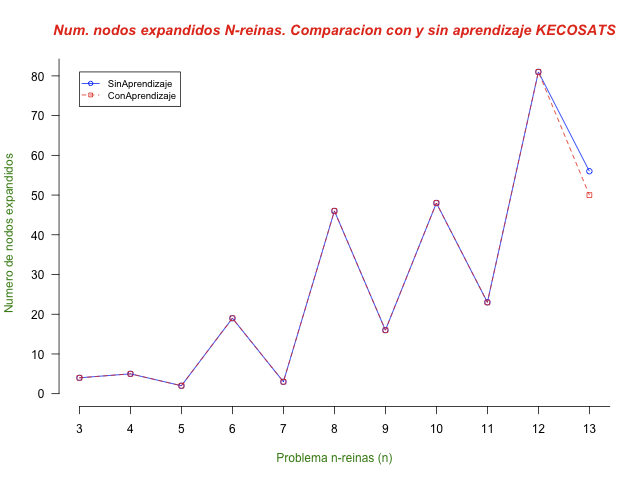
\includegraphics[scale=0.62]{figura21.png}
\end{figure}

\begin{figure}[!ht]\caption{Número de nodos expandidos en las N-reinas, para $14 \leq
    N \leq 17$}
\label{NodosExpandidosReinasPeq2}
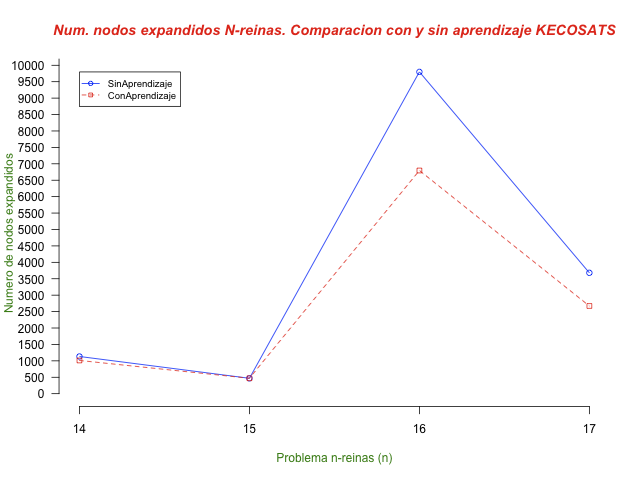
\includegraphics[scale=0.62]{figura22.png}
\end{figure}

\begin{figure}[!ht]\caption{Número de nodos expandidos en las N-reinas, para $18\leq
    N \leq 29$}
\label{NodosExpandidosReinasGrd}
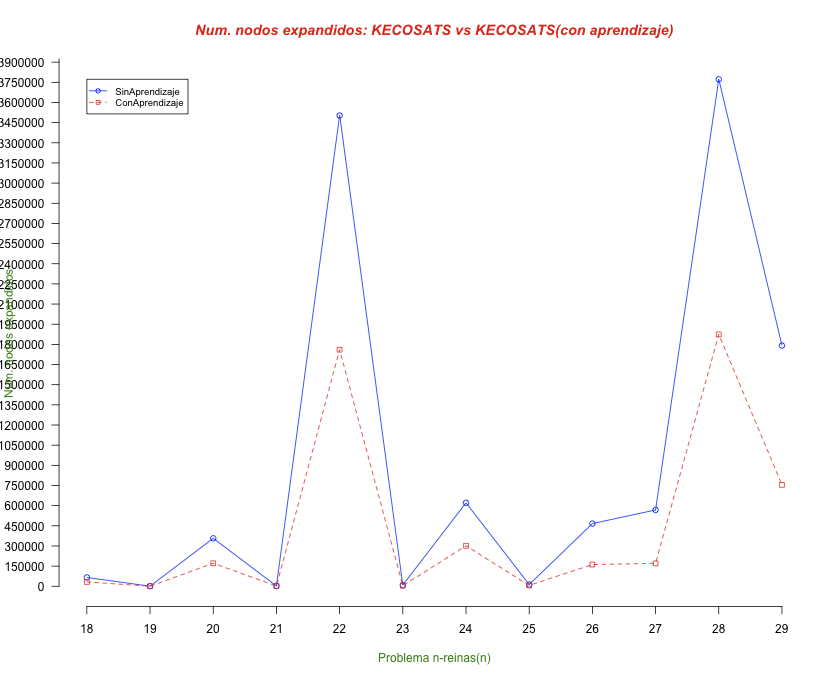
\includegraphics[scale=0.62,angle=90]{figura3.png}
\end{figure}

\begin{figure}[!ht]\caption{Número de saltos no cronológicos en las N-reinas}
\label{SaltosNCReinas}
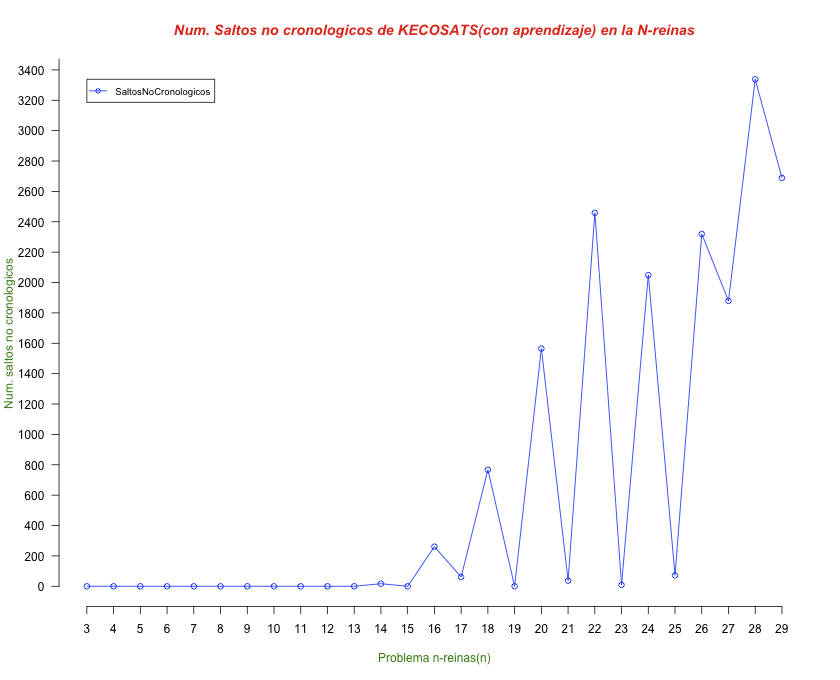
\includegraphics[scale=0.62,angle=90]{figura4.png}
\end{figure}

\newpage\newpage

\end{document}
